%%%%%%%%%%%%%%%%%%%%%%%%%%%%%%%%%%%%%%%%%
% Beamer Presentation
% LaTeX Template
% Version 1.0 (10/11/12)
%
% This template has been downloaded from:
% http://www.LaTeXTemplates.com
%
% License:
% CC BY-NC-SA 3.0 (http://creativecommons.org/licenses/by-nc-sa/3.0/)
%
%%%%%%%%%%%%%%%%%%%%%%%%%%%%%%%%%%%%%%%%%

%-------------------------------------------------------------------------------
%	PACKAGES AND THEMES
%-------------------------------------------------------------------------------

\documentclass{beamer}

\begin{filecontents}{\jobname.bib}

\end{filecontents}

\mode<presentation> {

% The Beamer class comes with a number of default slide themes
% which change the colors and layouts of slides. Below this is a list
% of all the themes, uncomment each in turn to see what they look like.
\usetheme{Madrid}
}

\usepackage{graphicx}
\usepackage{booktabs}
\usepackage{color, colortbl}
\usepackage{natbib}
\usepackage{setspace}
\usepackage[labelformat=simple]{caption}
\usepackage{tikz}

\usetikzlibrary{arrows,positioning,calc}

\definecolor{Lightgray}{rgb}{0.9, 0.9, 0.9}

%-------------------------------------------------------------------------------
%	TITLE PAGE
%-------------------------------------------------------------------------------

\title[]{Spanner: Google's Globally-Distributed Database}
\subtitle[]{}

\author{Kocher Daniel}

\institute[PLUS] 
{
Supervisor: Dipl.-Ing. Nikolaus Augsten, PhD \newline \newline \newline
University of Salzburg \\ 
\medskip
Daniel.Kocher@stud.sbg.ac.at
}
\date{\today}

\begin{document}
%-------------------------------------------------------------------------------
\begin{frame}
\titlepage
\end{frame}

%-------------------------------------------------------------------------------
\begin{frame}
\frametitle{Outline} 
\tableofcontents[hideallsubsections]
\end{frame}

%-------------------------------------------------------------------------------
\section{Motivation}
\begin{frame}
	\frametitle{Motivation}
	\begin{itemize}
    \item{Distributed data at global scale}
    \item{Externally-consistent distributed transactions}
    \item{High availability}
    \item{Two "competitors": \emph{Bigtable} \& \emph{Megastore}}
    \pause
    \item{Why not use Bigtable?}
    \begin{itemize}
      \item{Difficult to use for applications with complex, evolving schemas}
      \item{Only \emph{eventually-consistent} (no strong consistency)}
    \end{itemize}
    \pause
    \item{Why not use Megastore}
    \begin{itemize}
      \item{Poor write throughput}
    \end{itemize}
    
  \end{itemize}
\end{frame}

%-------------------------------------------------------------------------------
\begin{frame}
  \frametitle{Characteristics}
  \begin{center}
    \textbf{Spanner} evolved from a Bigtable-like versioned key-value store to a
    \textbf{temporal multi-version database}
  \end{center}
  \pause
  \begin{itemize}
    \item{Versioned data is stored in schematized semi-relational tables}
    \item{Each version is automatically timestamped with its commit time}
    \item{Garbage Collection \& Read at old timestamps}
    \item{\textbf{General-purpose transactions}}
    \item{SQL-like query language}
  \end{itemize}
\end{frame}

%-------------------------------------------------------------------------------
\begin{frame}
  \frametitle{Fundamentals}
  \begin{itemize}
    \item{Transaction $i$ is denoted $T_i$}
    %\item{RW \ldots Read-Write (transaction)}
    %\item{RO \ldots Read-Only (transaction)}
    \item{\textbf{Externally-consistent:} \newline
      If $T_1$ preceeds $T_2$ (Commit of $T_1$ happens before Begin of $T_2$, no
      overlap), then $T_1$ is serialized first
    }
    \pause
    \item{\textbf{Two-Phase Locking (2PL):} \newline
    Guarantees serializability
    \begin{enumerate}
      \item{\emph{Expanding} phase: locks are aquired, no locks are released}
      \item{\emph{Shrinking} phase: locks are released, no locks are aquired}
    \end{enumerate}
    }
    \item{\textbf{Two-Phase Commit (2PC):} \newline
    Coordinates processes participating in atomic distributed transaction
    \begin{enumerate}
      \item{\emph{Commit-Request} phase: Request "Yes" (Commit) or "No" (Abort) from
        every transaction process
      }
      \item{\emph{Commit} phase: Commit transaction if all voted "Yes", otherwise abort}
    \end{enumerate}
    }
  \end{itemize}
\end{frame}

%-------------------------------------------------------------------------------
\begin{frame}
  \frametitle{Features}
  As a globally-distributed database, Spanner provides interesting features:
  \begin{itemize}
    \item{Dynamically controlled replication configurations at fine grain}
    \item{Externally consistent reads \& writes}
    \item{globally-consistent reads at a timestamp}
  \end{itemize}
  $\Rightarrow$ enables \textbf{atomic schema changes} in presence of ongoing
  transactions \newline
  \pause
  \begin{itemize}
    \item{Timestamps reflect serialization order (linearizability)}
    \item{Key enabler: novel TrueTime API exposing clock uncertainty}
  \end{itemize}
\end{frame}

%-------------------------------------------------------------------------------
\section{Implementation}
\begin{frame}
  \frametitle{Implementation (Top-down)}
  \only<1-3>{
    \begin{itemize}
      \item{Spanner deployment is called \textbf{universe}}
      \item{Organized as a set of \textbf{zones}}
      \item{Zones are the unit of administrative deployment \& physical isolation}
      \item{Set of zones is the set of locations for replication}
      \pause
      \item{Each zone consists of}
      \begin{itemize}
        \item{several \textbf{spanservers} to store the data}
        \item{a \textbf{zonemaster} to assign data to spanservers}
        \item{a \textbf{location proxy} for clients to locate the assigned
          spanservers
        }
      \end{itemize}
      \pause
      \item{\textbf{universe master:} console to display status information about zones}
      \item{\textbf{placement driver:}}
      \begin{itemize}
        \item{handles automated data movement across zones}
        \item{moves data due to updated replication constraints or load balancing}
      \end{itemize}
    \end{itemize}
  }
  \only<4>{
    \begin{figure}
      \centering
      \includegraphics[width=.8\textwidth]{figures/spanner-server-organization.png}
      \caption{Spanner server organization}
    \end{figure}
  }
\end{frame}

%-------------------------------------------------------------------------------
\subsection{Spanserver Software Stack}
\begin{frame}
  \frametitle{Spanserver Software Stack}
  \only<1>{
    \begin{itemize}
      \item{Responsible for 100 - 1000 \textbf{tablets}}
      \item{A tablet is a bag of key-value mappings \newline
        \texttt{(key:string, timestamp:int64) $\rightarrow$ string}
      }
      \item{Timestamp are assigned to data $\Rightarrow$
        \textbf{multi-version database}
      }
      \item{Tablet states are stored on Colossus (successor of the GFS)}
      \item{Single Paxos state machine on top of each tablet to $\Rightarrow$
        \textbf{Replication}
      }
      \item{Set of replicas is called \textbf{Paxos group}}
    \end{itemize}
  }
  \pause
  \only<2>{
    \begin{itemize}
      \item{Every replica which is a leader implements}
      \begin{itemize}
        \item{a \textbf{lock table} for concurrency control: \texttt{(key range) $\rightarrow$ lock state}}
        \item{a \textbf{transaction manager} (TM) for distributed transactions}
      \end{itemize}
      \item{Transaction manager used to implement \textbf{participant leader}}
      \item{If multiple Paxos groups are involved: Two-Phase Commit}
      \begin{itemize}
        \item{One participant group is chosen as \textbf{coordinator}}
        \item{Participant leader of this group: \textbf{coordinator leader}}
      \end{itemize}
      \item{State of each Transaction manager is stored in Paxos group}
    \end{itemize}
  }
  \pause
  \only<3>{
    \begin{figure}
      \centering
      \includegraphics[width=.7\textwidth]{figures/spanserver-software-stack.png}
      \caption{Spanserver software stack}
    \end{figure}
  }
\end{frame}

%-------------------------------------------------------------------------------
\subsection{Directories \& Placement}
\begin{frame}
  \frametitle{Directories \& Placement}
  \only<1-4>{
    \begin{itemize}
      \item{\textbf{Directories:}}
      \begin{itemize}
        \item{Bucketing abstraction on top of key-value mappings}
        \item{Contain set of contiguous keys sharing common prefix}
        \item{Prefix allows to control locality of data}
        \item{Unit of data placement (same replication configuration)}
        \item{Smallest unit to specify geographic-replication properties (\textbf{placement})}
      \end{itemize}
      \pause
      \item{Data is moved directory-wise between Paxos groups}
      \item{Tablets may have multiple \textbf{partitions} of row space \newline
        $\Rightarrow$ co-locate directories frequently accessed together
      }
      \pause
      \item{Placements can be controlled in two dimensions:}
      \begin{enumerate}
        \item{Number \& types of replicas}
        \item{Geographic placement of replicas}
      \end{enumerate}
      \pause
      \item{\textbf{Movedir:} background task to move directories}
    \end{itemize}
  }
  \only<5>{
    \begin{figure}
      \centering
      \includegraphics[width=.6\textwidth]{figures/directories.png}
      \caption{Directories (the unit of data movement)}
    \end{figure}
  }
\end{frame}

%-------------------------------------------------------------------------------
\subsection{Data Model}
\begin{frame}
  \frametitle{Data Model}
  \only<1>{
    \begin{itemize}
      \item{Features:}
      \begin{itemize}
        \item{Schematized semi-relational tables}
        \item{SQL-like query language}
        \item{General-purpose transactions}
      \end{itemize}
      \item{Layered on top of directory-bucketed key-value mappings}
      \item{Applications create \textbf{databases} in universe}
      \item{Database may contain unlimited number of schematized \textbf{tables}}
      \item{Table contains rows (must have names), columns \& versioned values}
    \end{itemize}
  }
  \only<2>{
    \begin{figure}
      \centering
      \includegraphics[width=.5\textwidth]{figures/interleaving-example.png}
      \caption{Interleaving example}
    \end{figure}
    \begin{itemize}
      \item{Interleaving of tables to form directories is significant}
      \item{Locality relationships between multiple tables $\Rightarrow$ good
        performance
      }
    \end{itemize}
  }
\end{frame}

%-------------------------------------------------------------------------------
\section{TrueTime}
\begin{frame}
  \frametitle{TrueTime}
  \only<1>{
    \begin{table}
      \centering
      \begin{tabular}{|l||l|}
        \hline
        Method & Returns \tabularnewline
        \hline\hline
        $TT.now()$ & $TTinterval$: [$earliest$, $latest$] \tabularnewline
        \hline
        $TT.after(t)$ & true if $t$ has definitely passed \tabularnewline
        \hline
        $TT.before(t)$ & true if $t$ has definitely not arrived \tabularnewline
        \hline
      \end{tabular}
      \caption{TrueTime API ($t$ is of type $TTstamp$)}
    \end{table}
    Time is represented as a $TTinterval$ (interval with bounded uncertainty)
    \newline\newline
    Let $e$ be an event and $t_{abs}(e)$ denote the absolute time of $e$.
    \newline
    For $tt = TT.now()$, the following property holds:
    \begin{center}
      $tt.earliest \leq t_{abs}(e) \leq tt.latest$
    \end{center}
  }
  \only<2>{
    \begin{figure}
      \centering
      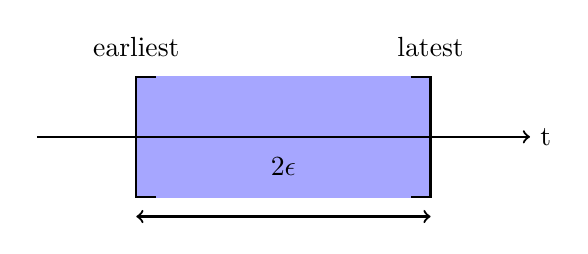
\begin{tikzpicture}[thick]
        \node (left-end) at (0, 0) {};
        \node[right = 6 of left-end] (right-end) {};

        \node[right = 1 of left-end] (left-bound) {};
        \node[left = 1 of right-end] (right-bound) {};

        \node[above = 0.5 of left-bound] (left-bound-top) {};
        \node[below = 0.5 of left-bound] (left-bound-bottom) {};
        \node[above = 0.5 of right-bound] (right-bound-top) {};
        \node[below = 0.5 of right-bound] (right-bound-bottom) {};

        \draw[blue!35, fill=blue!35] (left-bound-top.center) rectangle (right-bound-bottom.center);
        \node (two-e-invis) at ($(left-bound.south)!0.5!(right-bound.south)$) {};
        \node[below = 0 of two-e-invis.center] (two-e-t) {$2\epsilon$};
        \draw[->] (left-end.center) -- (right-end.center) node[right] {t};

        \draw (left-bound.center) -- (left-bound-top.center) -- ++(0.25, 0);
        \draw (left-bound.center) -- (left-bound-bottom.center) -- ++(0.25, 0);
        \draw (right-bound.center) -- (right-bound-top.center) -- ++(-0.25, 0);
        \draw (right-bound.center) -- (right-bound-bottom.center) -- ++(-0.25, 0);

        \node[above = 0 of left-bound-top.north] (left-bound-t) {earliest};
        \node[above = 0 of right-bound-top.north] (right-bound-t) {latest};

        \node[below = 0.75 of left-bound] (left-bound-e) {};
        \node[below = 0.75 of right-bound] (right-bound-e) {};

        \draw[<->] (left-bound-e.center) -- (right-bound-e.center);
        %\node[below right= 1 and 2.5 of left] {$2\epsilon$};
      \end{tikzpicture}
      \caption{Visualization of $TT.now()$ and $\epsilon$}
    \end{figure}
  }
  \only<3>{
    \begin{itemize}
      \item{Time references: GPS and atomic clocks (different failure modes)}
      \item{Set of \textbf{time master} machines per datacenter}
      \item{\textbf{Armageddon masters}: masters using atomic clocks}
      \item{\textbf{timeslave daemon} per machine}
      \pause
      \item{Masters compare their time references regularly}
      \item{Daemons poll a variety of masters (liar detection)}
      \pause
      \item{$\epsilon$ is the instantaneous error bound (typically 1 - 7ms)}
      \item{$\overline{\epsilon}$ is the average error bound (typically 4ms)}
      \item{$\epsilon$ is derived from applied worst-case local clock drift ($200\mu s/sec$)}
    \end{itemize}
  }
\end{frame}

%-------------------------------------------------------------------------------
\section{Concurrency Control}
\begin{frame}
  \frametitle{Concurrency Control}
  \begin{itemize}
    \item{TrueTime is used to guarantee correctness properties}
    \item{Properties are used to implement}
    \begin{itemize}
      \item{Externally-consistent transactions}
      \item{Lock-free read-only transactions}
      \item{Non-blocking reads in the past}
    \end{itemize}
  \end{itemize}
\end{frame}

%-------------------------------------------------------------------------------
\subsection{Timestamp Management}
\begin{frame}
  \frametitle{Timestamp Management}
  \only<1>{
    \footnotesize
    \begin{table}
      \begin{tabular}{|l||l|l|}
        \hline
        Operation & CC & Replica required\tabularnewline
        \hline\hline
        Read-Write transaction & Pessimistic & leader\tabularnewline
        \hline
        Read-Only transaction & Lock-free & leader; any
        \tabularnewline
        \hline
        Snapshot Read, client-provided timestamp & Lock-free & any\tabularnewline
        \hline
        Snapshot Read, client-provided bound & Lock-free & any \tabularnewline
        \hline
      \end{tabular}
      \caption{Supported types of reads \& writes}
    \end{table}
  }
  \begin{itemize}
    \item{Standalone write $\Rightarrow$ RW transaction}
    \item{Non-snapshot standalone read $\Rightarrow$ RO transaction}
    \item{RO transactions}
    \begin{itemize}
      \item{must predeclare to not include writes}
      \item{can proceed on any sufficiently up-to-date-replica (also snapshot reads)}
    \end{itemize}
  \end{itemize}
\end{frame}

%-------------------------------------------------------------------------------
\subsubsection{Paxos Leader Leases}
\begin{frame}
  \frametitle{Paxos Leader Leases}
  \begin{itemize}
    \item{Timed leases for long-lived leadership (10s by default)}
    \item{Quorum of lease votes $\Rightarrow$ leader has a lease}
    \item{Successful writes extend lease vote on replica}
    \item{\textbf{Disjointness invariant:} \newline
      For each Paxos group, each Paxos leader's \emph{lease interval} is disjoint
      from every other leader's
    }
    \item{Leaders must not abdicate before $TT.after(s_{max})$, where $s_{max}$
      denotes the maximum timestamp used by a leader
    }
  \end{itemize}
\end{frame}

%-------------------------------------------------------------------------------
\subsubsection{Timestamps in RW Transactions}
\begin{frame}
  \frametitle{Timestamps in RW Transactions}
  \begin{itemize}
    \item{Timestamp assignment only in between the two phases (2PL)}
    \item{\textbf{Monotonicity variant:} \newline
      Within each Paxos group, Spanner assigns timestamps to Paxos writes in
      monotonically increasing order, even across leaders
    }
    \item{Enforced across leaders by disjointness invariant: \newline
      Leader must only assign timestamps within the interval of leader lease
    }
    \item{Timestamp $s$ assigned $\Rightarrow$ $s_{max} = s$}
    \item{\textbf{External consistency invariant}: \newline
      \begin{center}
        $t_{abs}\left(e^{commit}_1\right) < t_{abs}\left(e^{start}_2\right)$
        $\Rightarrow s_1 < s_2$
      \end{center}
    }
  \end{itemize}
\end{frame}

%-------------------------------------------------------------------------------
\subsubsection{Serving Reads at a Timestamp}
\begin{frame}
  \frametitle{Serving Reads at a Timestamp}
  \begin{itemize}
    \item{Monotonicity invariant allows to determine if a replica's state is
      \textbf{sufficiently up-to-date} to satisfy a read
    }
    \item{\textbf{Safe time} $t_{safe}$ at each replica}
    \item{Replica satisfies read if $t \leq t_{safe}$}
    \item{$t_{safe} = min\left(t^{Paxos}_{safe}, t^{TM}_{safe}\right)$}
  \end{itemize}
\end{frame}

%-------------------------------------------------------------------------------
\subsubsection{Timestamps in RO Transactions}
\begin{frame}
  \frametitle{Timestamps in RO Transactions}
  \begin{itemize}
    \item{Two phases:}
    \begin{enumerate}
      \item{Assign timestamp $s_{read}$}
      \item{Execute transaction's reads as snapshot reads at $s_{read}$}
    \end{enumerate}
    \item{Spanner assigns the oldest timestamp that preserves external consistency
      to reduce the changes of blocking
    }
  \end{itemize}
\end{frame}

%-------------------------------------------------------------------------------
\subsection{Details}

\subsubsection{Read-Write Transactions}
\begin{frame}
  \frametitle{Read-Write Transactions}
  \begin{itemize}
    \item{RW transactions buffered at client until Commit}
    \item{Reads do not see effects of transaction's writes}
    \item{Client has completed all reads \& buffered all writes $\Rightarrow$ 2PC}
    \pause
    \item{Non-coordinator-participant leader}
    \begin{enumerate}
      %\item{Acquires write locks}
      \item{Chooses prepare timestamp according to monotonicity}
      \item{Logs prepare record through Paxos}
      \item{Notifies coordinator of its prepare timestamp}
    \end{enumerate}
    \pause
    \item{Coordinator leader}
    \begin{enumerate}
      %\item{Aquires write locks}
      \item{Chooses timestamp for whole transaction}
      \item{Commit timestamp $s$ must be}
      \begin{itemize}
        \item{$\geq$ all prepare timestamps}
        \item{$> TT.now().latest$ at the time the Commits were received}
        \item{$>$ any previously assigned timestamp}
      \end{itemize}
      \item{Logs Commit record through Paxos}
    \end{enumerate}
  \end{itemize}
\end{frame}

%-------------------------------------------------------------------------------
\subsubsection{Read-Only Transactions}
\begin{frame}
  \frametitle{Read-Only Transactions}
  \begin{itemize}
    \item{\textbf{scope} expression summarizing the keys that will be read}
    \item{Served by single Paxos group \newline
      $\Rightarrow$ client issues transaction to group leader
    }
    \item{Served by multiple Paxos groups \newline
      $\Rightarrow$ client executes reads at $s_{read} = TT.now().latest$
    }
    \item{All reads can be sent to replicas that are sufficiently up-to-date}
  \end{itemize}
\end{frame}

%-------------------------------------------------------------------------------
\subsubsection{Schema-Change Transactions}
\begin{frame}
  \frametitle{Schema-Change Transactions}
  \begin{itemize}
    \item{TrueTime enables this feature}
    \item{Use of standard transaction infeasible}
    \item{Non-blocking variant of standard transaction}
    \begin{enumerate}
      \item{Explicit assignment of a future timestamp (Prepare phase)}
      \item{Reads \& writes synchronize with any registered schema-change
        timestamp at time $t$
      }
    \end{enumerate}
    \item{Without TrueTime $\Rightarrow$ schema change at $t$ would be meaningless
    }
  \end{itemize}
\end{frame}

%-------------------------------------------------------------------------------
%\subsubsection{Refinements}
%\begin{frame}
%  \frametitle{Refinements}
%  \begin{itemize}
%    \item{}
%  \end{itemize}
%\end{frame}

%-------------------------------------------------------------------------------
\section{Evaluation}

\subsection{Microbenchmarks}
\begin{frame}
  \frametitle{Microbenchmarks}
  \only<1>{
    \begin{itemize}
      \item{Setup:}
      \begin{itemize}
        \item{4GB RAM scheduling units per spanserver}
        \item{4 cores (AMD Barcelona 2200MHz) per spanserver}
        \item{One spanserver per zone}
        \item{Clients \& zones in set of datacenters with network distance $<$ 1ms}
        \item{Database created with 50 Paxos groups with 2500 directories}
      \end{itemize}
      \item{Operations: standalone reads \& writes of 4KB}
      \item{One unmeasured round of reads to warm any location caches}
    \end{itemize}
  }
  \only<2>{
    \textbf{Latency [ms] (less is better)}
    \begin{table}
      \centering
      \begin{tabular}{|l||l|l|l|}
        \hline
        Replicas & Write & RO Transaction & Snapshot Read \tabularnewline
        \hline\hline
        1D & $9.4\pm0.6$ & - & - \tabularnewline
        \hline
        1 & $14.4\pm1.0$ & $1.4\pm0.1$ & $1.3\pm0.1$ \tabularnewline
        \hline
        3 & $13.9\pm0.6$ & $1.3\pm0.1$ & $1.2\pm0.1$ \tabularnewline
        \hline
        5 & $14.4\pm0.4$ & $1.4\pm0.05$ & $1.3\pm0.04$ \tabularnewline
        \hline
      \end{tabular}
      \caption{Latency experiments}
    \end{table}
    \begin{itemize}
      \item{Sufficiently few operations to avoid queuing}
      \item{Increasing number of replicas:}
      \begin{itemize}
        \item{Latency stays roughly constant with less standard deviation}
        \item{Latency to achieve quorum less sensitive to stragglers}
      \end{itemize}
    \end{itemize}
  }
  \only<3>{
    \textbf{Throughput [Kops/sec] (more is better)}
    \begin{table}
      \centering
      \begin{tabular}{|l||l|l|l|}
        \hline
        Replicas & Write & RO Transaction & Snapshot Read \tabularnewline
        \hline\hline
        1D & $4.0\pm0.3$ & - & - \tabularnewline
        \hline
        1 & $4.1\pm0.05$ & $10.9\pm0.4$ & $13.5\pm0.1$ \tabularnewline
        \hline
        3 & $2.2\pm0.5$ & $13.8\pm3.2$ & $38.5\pm0.3$ \tabularnewline
        \hline
        5 & $2.8\pm0.3$ & $25.3\pm5.2$ & $50.0\pm1.1$ \tabularnewline
        \hline
      \end{tabular}
      \caption{Throughput experiments}
    \end{table}
    \begin{itemize}
      \item{Sufficiently many operations to saturate servers' CPUs}
      \item{Increasing number of replicas:}
      \begin{itemize}
        \item{Snapshot read throughput increases almost linear}
      \end{itemize}
    \end{itemize}
  }
\end{frame}

%-------------------------------------------------------------------------------
\subsection{Availability}
\begin{frame}
  \frametitle{Availability}
  \only<1>{
    \begin{itemize}
      \item{Setup:}
      \begin{itemize}
        \item{Universe with 5 zones $Z_i$, each of which has 25 spanservers}
        \item{Database sharded into 1250 Paxos groups}
        \item{100 clients constantly issued snapshot reads (50K reads/sec)}
        \item{All leaders explicitly place in $Z_1$}
        \item{5s into each test, all servers in one zone were killed}
      \end{itemize}
    \end{itemize}
  }
  \only<2>{
    \begin{figure}
      \centering
      \includegraphics[width=.5\textwidth]{figures/effect-of-killing-servers-on-throughput.png}
      \caption{Effect of killing servers on throughput}
    \end{figure}
    \begin{itemize}
      \item{Availability benefits of running Spanner in multiple datacenters}
      %\item{Killing $Z_2$ (non-leader): no effect on read throughput}
      %\item{Killing $Z_1$ with notifications (leader-soft): minor effect}
      %\item{Killing $Z_1$ without notifications (leafer-hard): severe effect}
    \end{itemize}
  }
\end{frame}

%-------------------------------------------------------------------------------
\subsection{TrueTime}
\begin{frame}
  \frametitle{TrueTime}
  \begin{itemize}
    \item{Two questions:}
    \begin{itemize}
      \item{Is $\epsilon$ truly a bound on clock uncertainty?}
      \item{How bad does $\epsilon$ get?}
    \end{itemize}
    \pause
    \item{Answers:}
    \begin{itemize}
      \item{Clock issues infrequent relative to more serious hardware problems
      \newline $\Rightarrow$ TrueTime as trustworthy as any other piece of software
      }
    \end{itemize}
    \pause
    \begin{figure}
      \centering
      \includegraphics[width=.6\textwidth]{figures/epsilon.png}
      \caption{Distribution of TrueTime $\epsilon$ values}
    \end{figure}
  \end{itemize}
\end{frame}

%-------------------------------------------------------------------------------
\section{Conclusions \& Future Work}
\begin{frame}
  \frametitle{Conclusions \& Future Work}
  \begin{itemize}
    \item{5 years from Spanner's inception to iterate to the current design}
    \item{Combines \& extends on ideas from database \& systems community}
    \item{Linchpin: TrueTime}
    \item{Build distributed systems with much stronger time semantics}
    \item{No longer depend on loosely synchronized clocks \& weak time APIs}
    \pause
    \item{Future Work:}
    \begin{itemize}
      \item{Implement optimistical reads in parallel}
      \item{Support direct changes of Paxos configurations}
      \item{Improve single-node performance}
      \item{Support movement of processes between datacenters}
    \end{itemize}
  \end{itemize}
\end{frame}

%-------------------------------------------------------------------------------
\begin{frame}
	\frametitle{Thank you for your attention!}
	\begin{center}
		\huge{Questions?}
	\end{center}
	%\par{References: \tiny{
	%	\def\newblock{\hskip .11em plus .33em minus .07em}
	%	\bibliography{\jobname}
	%	}
	%}
\end{frame}

\end{document} 
